% Befehl \fibelvorstellung: Erstellt die Vorstellung eines FSlers mit Bild
%	Parameter #1: Bild (wrapfigure)
%	Parameter #2: Text
\newcommand{\fibelvorstellung}[2]{%
	\begin{minipage}{\columnwidth}
		% Kein Abstand vor bzw. nach Bildern bei wrapfigure
		\setlength{\intextsep}{0cm}
		% geringfügiger Abstand zwischen Paragraphen
		\setlength{\parskip}{0.5ex}
		#1
		#2
		\vspace{0.5ex}
	\end{minipage}
	
	\vspace{5ex plus 2ex minus 1ex}
}
\newlength{\fibelstdlen}
\setlength{\fibelstdlen}{3.7cm}

\section{Der Fachschaftsrat~(FSR) Physik stellt sich vor}
\begin{multicols}{2}
\small


\fibelvorstellung{
	\begin{wrapfigure}{l}{0cm}
		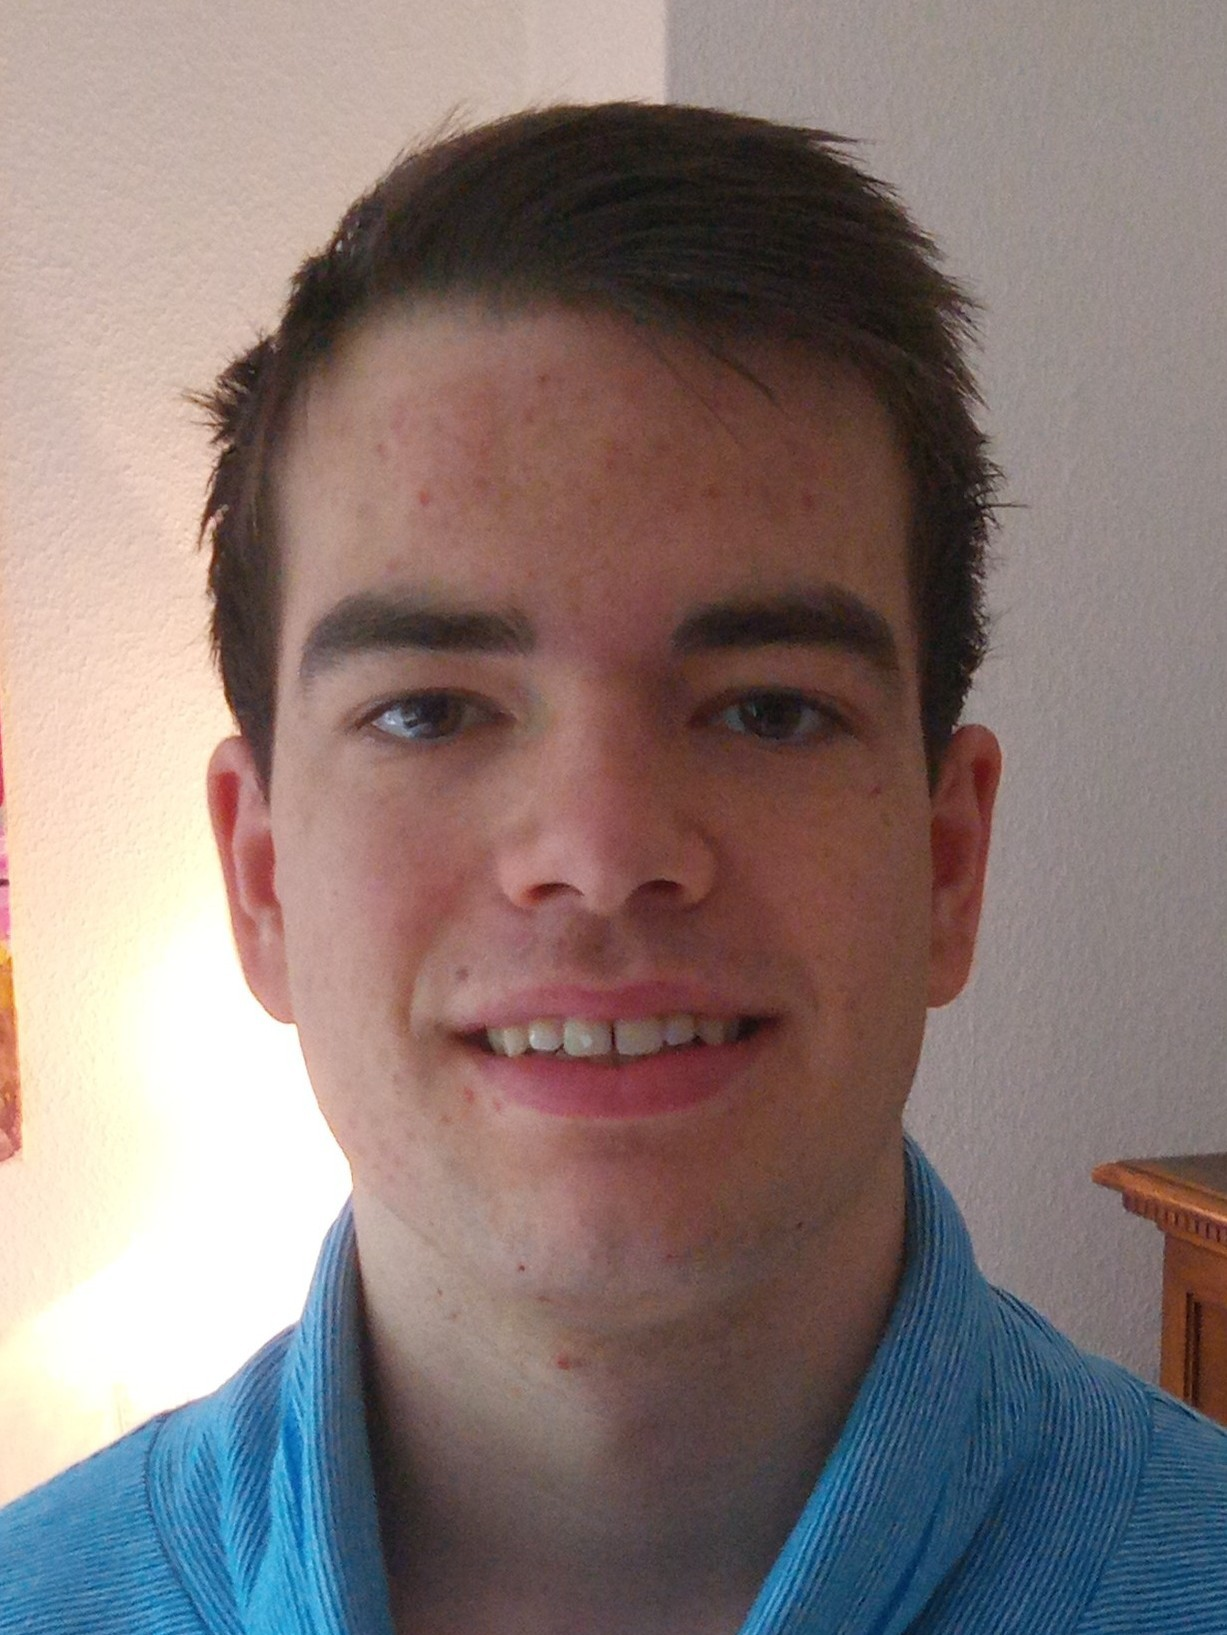
\includegraphics[width=\fibelstdlen]{res/vorstellungsfotos/Fotos Selbstvorstellungstexte Fibel/Lambert.jpg}
	\end{wrapfigure}
}
{
Hallo, ich bin Lambert und fange in diesem Semester meine Masterarbeit an. Aktuell bin ich Vorsitzender der Fachschaft, mitverantwortlich für die Evaluation der Lehre, den BaMa-Tag und bin in fast allen Gremien des Fachbereichs. Abseits der Uni lese ich gerne und spiele Tischtennis. Mit Fragen zum 1-Fach-Bachelor allgemein und den meisten Nebenfächern sowie allem anderen was euch einfällt, könnt ihr euch gerne an mich wenden. Willkommen in Münster! 
}

\vspace{-0.5cm}

\fibelvorstellung{
	\begin{wrapfigure}{r}{0cm}
		\includegraphics[width=\fibelstdlen]{res/vorstellungsfotos/Hauke_neu.jpg}
	\end{wrapfigure}
}
{
Moin, ich heiße Hauke und bin seit 2016 an der Uni und in der Fachschaft. Als Erasmus Student war ich in Sevilla (Spanien) und in Münster bin ich für die Evaluation der Lehre zuständig. Mittlerweile schreibe ich meine Masterarbeit in der Geophysik. 
Euch ein herzliches Willkommen in Münster!
}

\vspace{-0.5cm}

\fibelvorstellung{
	\begin{wrapfigure}{l}{0cm}
		\includegraphics[width=\fibelstdlen]{res/vorstellungsfotos/Tim.jpg}
	\end{wrapfigure}
}
{
Hej, ich bin Tim und arbeite als Doktorand am Institut für Kernphysik. In der Fachschaft bin ich hauptsächlich für die Finanzen zuständig. Ihr könnt gerne mit Fragen rund ums Studium zu mir kommen, auch und insbesondere, wenn ihr euch für einen Auslandsaufenthalt interessiert. Ich habe nämlich selbst ein Jahr mit Erasmus in Schweden verbracht. Aber erstmal wünsche ich euch viel Spaß in der O-Woche und hoffe, dass ihr viele andere Erstis kennen lernt. Vielleicht läuft man sich ja mal in der Uni über den Weg, zum Beispiel beim Spieleabend der Fachschaft. :) 
}

\fibelvorstellung{
	\begin{wrapfigure}{l}{0cm}
		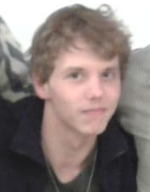
\includegraphics[width=\fibelstdlen]{res/vorstellungsfotos/Marius_cut.PNG}
	\end{wrapfigure}
}
{
Hi, ich bin Marius und heiße euch ebenfalls herzlich willkommen hier in Münster. Wenn ihr die Stadt noch nicht richtig kennt, dann freut euch darauf, sie kennenzulernen. 
Das Studium wird zwar zwischendurch hart, aber lasst euch trotzdem nicht die Freude dran nehmen. ¡Mucha suerte!\footnote{\url{https://www.youtube.com/watch?v=iik25wqIuFo}}
}


\vspace{-0.4cm}

\fibelvorstellung{
	\begin{wrapfigure}{l}{0cm}
		\includegraphics[width=\fibelstdlen]{res/vorstellungsfotos/Christoph.PNG}
	\end{wrapfigure}
}
{
Sehr geehrte Erstis: Moin!
Ich bin Christoph und studiere im Master Physik. In der Fachschaft bin ich im O-Wochen Team und beim Sommerfest tätig. Wenn Ihr Fragen habt, z.B zur O-Woche oder zum etwas Chaotischen Alltag an der Uni, immer her damit, es lebe das Chaos! :D 
Ich wünsche euch allen eine schöne O-Woche und hoffe man sieht sich mal in der Fachschaft.
}

\vspace{-0.5cm}

\fibelvorstellung{
	\begin{wrapfigure}{r}{0cm}
		\includegraphics[width=\fibelstdlen]{res/vorstellungsfotos/Alexander_T_cut.jpg}
	\end{wrapfigure}
}
{
Hi, ich bin Alexander und studiere hier Physik im Master. Ich organisiere unter Anderem die Ersti-Fahrt und bin für die IT zuständig. 
Ich heiße euch herzlich willkommen an der Uni Münster und wünsche einen guten Start in das Studium!
}

%\vspace{-1.5cm}

\fibelvorstellung{
	\begin{wrapfigure}{l}{0cm}
		\includegraphics[width=\fibelstdlen]{res/vorstellungsfotos/Jasemin.jpg}
	\end{wrapfigure}
}
{
Hey\textasciicircum\textasciicircum \\
Ich bin Jasemin, studiere Physik und Sozialwissenschaften auf Lehramt und bin aktuell am Ende meines Bachelors. In der Fachschaft kümmere ich mich um die Ersti-Fahrt, O-Woche und Gremienarbeit. Wenn ihr also Fragen oder Vorschläge für Aktivitäten für euch Erstis habt, meldet euch gerne bei mir. 
Ich wünsche euch viel Spaß in eurem ersten Semester des Physik-Studiums.
}

%\vspace{-1.2cm}

\fibelvorstellung{
	\begin{wrapfigure}{l}{0cm}
		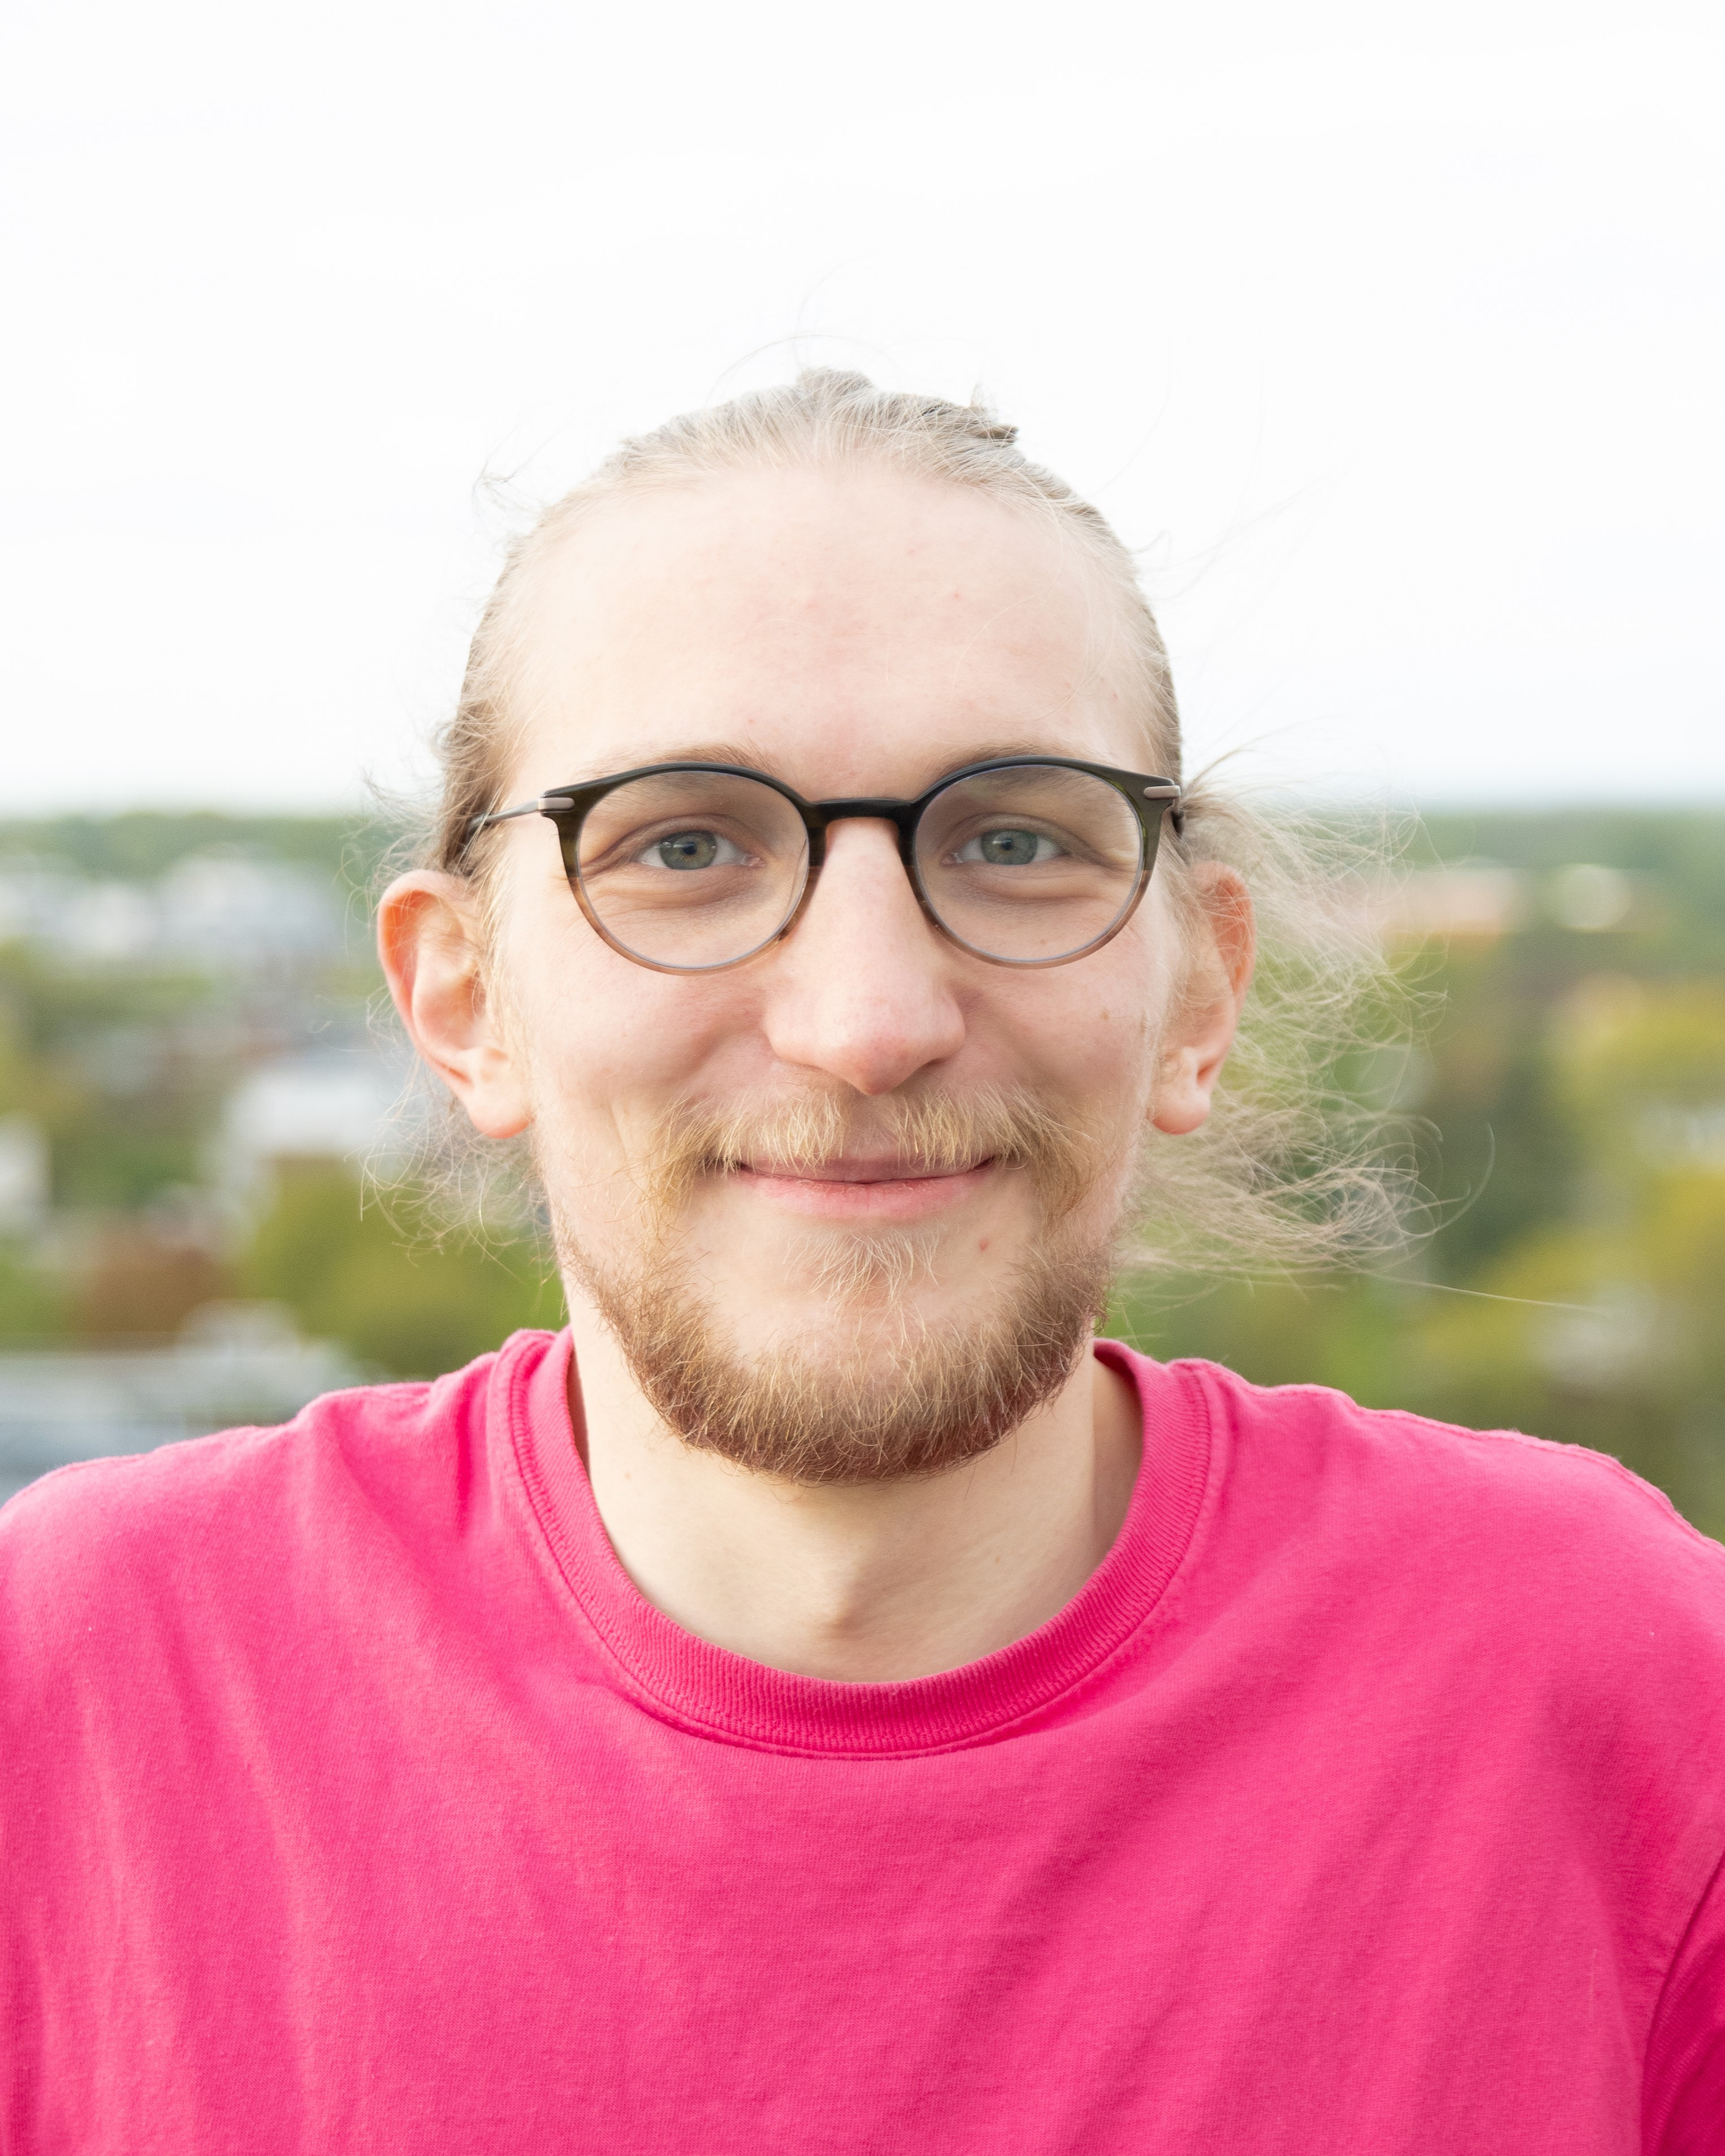
\includegraphics[width=\fibelstdlen]{res/vorstellungsfotos/Moritz.jpg}
	\end{wrapfigure}
}
{
Hi, ich bin Maurice, gerade im Übergang zum Master of Education und schon seit einigen Jahren in der Fachschaft dabei. Aktuell bin ich Vorsitz der FSV (eine der vielen verwirrenden Abkürzungen aus dem Artikel zur Hochschulpolitik) und im Social-Media-Team. Außerdem dürfen mich alle Zweifachbachelor gerne mit ihren Fragen zum Studium löchern. Ich wünsche euch allen einen spannenden und Studienstart und denkt daran, der Artikel "Das große Bluffspiel" seht nicht umsonst in dieser Fibel.
}

% \vspace{-0.3cm}

\fibelvorstellung{
	\begin{wrapfigure}{l}{0cm}
		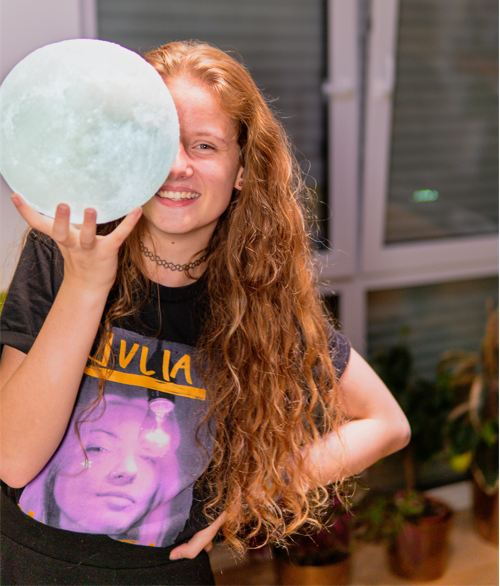
\includegraphics[width=\fibelstdlen]{res/vorstellungsfotos/Eva_cut.PNG}
	\end{wrapfigure}
}
{
Hey, ich heiße Eva und studiere Physik im Master. Seit dem Sommersemester 2020 bin ich in der Fachschaft und betätigte mich im Design-Team und in der Öffentlichkeitsarbeit.
Ich wünsche Euch einen tollen Start ins Studium! \\ PS: Über ein freundliches „Hallo“ (auf dem Gang, im Vorbeigehen) freue ich mich immer.
} 

\vspace{-0.8cm}

\fibelvorstellung{
	\begin{wrapfigure}{r}{0cm}
		\includegraphics[width=\fibelstdlen]{res/vorstellungsfotos/Philipp_cut.JPG}
	\end{wrapfigure}
}
{
Moin! Ich bin der Phil, und kurz davor den Bachelor abzuschließen.
In der Fachschaft bin ich seit über drei Jahren aktiv und kümmere mich hier hauptsächlich um interne Angelegenheiten.
Ich wünsche euch eine schöne O-Woche und ein guten Start in das Studium.
}

%\vspace{0.1cm}

%\vspace{0.1cm}

\fibelvorstellung{
	\begin{wrapfigure}{l}{0cm}
		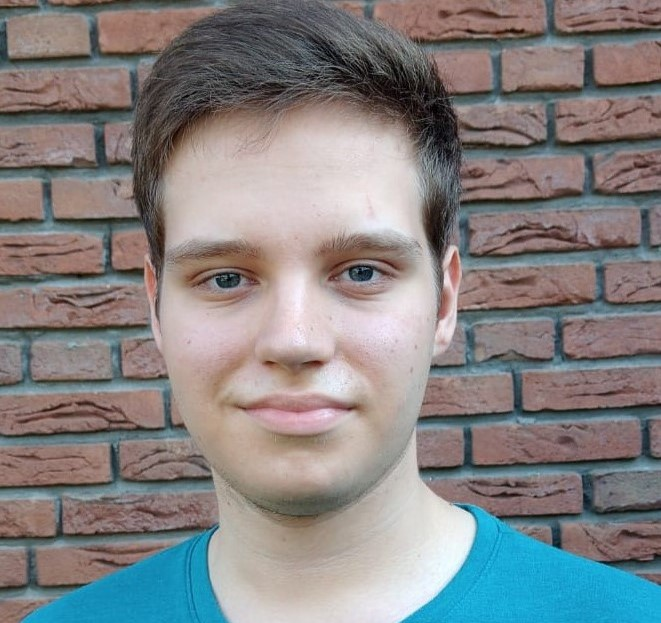
\includegraphics[width=\fibelstdlen]{res/vorstellungsfotos/Phillip_S_cut.jpg}
	\end{wrapfigure}
}
{
Moin, ich bin Phillip und studiere im 5. Semester Physik. In der Fachschaft bin ich für den Hochschultag verantwortlich. Ich wünsche euch eine schöne O-Woche und viel Spaß in Münster und beim Studium. 
}

\vspace{-0.3cm}

\fibelvorstellung{
	\begin{wrapfigure}{l}{0cm}
		\includegraphics[width=\fibelstdlen]{res/vorstellungsfotos/Marc.jpg}
	\end{wrapfigure}
}
{
Moin! Ich bin Marc und studiere seit 2022 1-Fach Bachelor Physik an der WWU und bin quasi direkt der Fachschaft beigetreten. Ich helfe hier bei der Evaluation der Lehre mit. Mit Fragen könnt ihr sehr gerne zu mir kommen! Insbesondere über mein Nebenfach "Spanisch für Naturwissenschaftler" kann ich euch mittlerweile ein wenig was erzählen. Ich wünsche euch einen tollen Start in euer Studium!!! 
} 

\vspace{-0.5cm}

\fibelvorstellung{
	\begin{wrapfigure}{r}{0cm}
		\includegraphics[width=\fibelstdlen]{res/vorstellungsfotos/Hannes.png}
	\end{wrapfigure}
}
{
Hey, ich bin Hannes und studiere gerade im 5. Semester. Als Nebenfach mache ich Psychologie. In der Fachschaft bin ich unter Anderem bei der Planung des Sommerfests und der Erstifahrt mit eingebunden. Mein Tipp: Sucht euch Leute, mit denen ihr die gemeinsam lernt. Das ist m.\,M.\ nach das Wichtigste zum Start! Ansonsten, gebt nicht zu schnell auf. Auch wenn es am Anfang manchmal durchaus frustrierend sein kann.
Falls ihr fragen rund ums Studium habt, sprecht mich gerne an wenn ihr mich seht. :D 
Viel Erfolg!
}

\fibelvorstellung{
	\begin{wrapfigure}{l}{0cm}
		\includegraphics[width=\fibelstdlen]{res/vorstellungsfotos/Saba.jpg}
	\end{wrapfigure}
}
{
Hi, ich bin Saba Ahmed Cheema und studiere Physik auf Master. Zur Zeit bin ich auch Mitglied einer Berufungskommission einer Professur zur Photonik. Ich wünsche euch einen guten Start in's Studium. 
}



%
% \begin{center}
% 	\includegraphics[width=\columnwidth]{res/fsphys_logo.pdf}
% \end{center}
%
%
%

% \vspace{6ex}

% \fibelvorstellung{
% 	\begin{wrapfigure}{r}{0cm}
% 		\includegraphics[width=\fibelstdlen]{res/vorstellungsfotos/fritz.png}
% 	\end{wrapfigure}
% }
% {
% Hallo, ich bin Fritz und bin schon  in der Fachschaft Physik.
% Die Mannschaft hier ist echt genial aufgestellt. Dadurch macht es richtigen Spaß, ein aktiver Teil der Universität % Münster zu sein.
% Ich kann dir nur empfehlen: Mach' mit und verändere die Uni!
% }


\end{multicols}

% \vspace{20ex}
